\documentclass[10pt,a4paper]{article}

\usepackage[utf8]{inputenc}
\usepackage[T1]{fontenc}
\usepackage[english]{babel}
\usepackage{lmodern}
\usepackage{microtype}
\usepackage[top=1.5cm, bottom=1.5cm, left=1.7cm, right=1.7cm]{geometry}
\usepackage{graphicx}
\graphicspath{{figures/}}
\usepackage{xcolor}
\definecolor{navyblue}{RGB}{0, 45, 110}
\usepackage[colorlinks=true, linkcolor=navyblue, urlcolor=navyblue]{hyperref}
\usepackage[capitalise]{cleveref}
\usepackage{enumitem}
\setlist{nosep, leftmargin=*, itemsep=2pt}
\usepackage[font=small, labelfont=bf, skip=3pt]{caption}
\usepackage{tikz}
\usetikzlibrary{positioning, arrows.meta}
\pagestyle{empty}
\setlength{\parindent}{0pt}

\newcommand{\us}{\textbf{Us}}
\newcommand{\cl}{\textbf{Claude}}

\begin{document}
\begin{center}
  {\Large\bfseries How we used AI}\\[2pt]
  Matteo Nizard, Norman El Fartass \quad--\quad companion note to the DAgger vs RLPD report
\end{center}

We used Claude (Claude Code) as a \emph{tutor}, an \emph{implementer} of code we had first written and understood,
a \emph{reviewer}, and above all a \emph{job manager} for our experiments. Questions, choices and conclusions were
ours. In chronological order:

\begin{enumerate}
  \item \textbf{Understanding the problem.} \us: re-read DAgger, explored the project template.
        \cl: explained DAgger and RLPD in detail, revised SAC with us.
  \item \textbf{First simulations.} \cl: set up the environment and the scripts to explore observations and
        compare the experts. \us: decided what to measure.
  \item \textbf{Choices, brainstorm between us} (\cref{fig:board}), then reviewed by Claude: continuous actions only,
        so team~4 alone to start; one simple training track (lighthouse) and two held-out test tracks.
  \item \textbf{Algorithms.} \us: wrote DAgger and RLPD (on top of SAC), had them reviewed elsewhere.
        \cl: once we understood them, implemented them in the project, then corrected and compacted; we re-read it.
  \item \textbf{Smoke tests.} \us: found the problems and chose the answers (normalisation, DAgger saturating,
        RLPD reward hack $\to$ reward cap, RLPD not generalising). \cl: made the fixes.
  \item \textbf{Where AI helped most: night-time job manager} (\cref{fig:jobs}). \cl: launched, watched, fixed and
        relaunched runs on our two laptops and Kaggle, and wrote each experiment's tables \emph{without conclusions}.
        \us: in the morning, analysed unbiased reports and real statistics.
  \item \textbf{Last corrections.} \us: spotted two gaps, an expert-free baseline (SAC alone) and noise on DAgger.
        \cl: relaunched them. \us: analysed.
  \item \textbf{Report.} \us: wrote the whole draft in French. \cl: checked it against the logs, then wrote the
        English \LaTeX{} and the figures.
\end{enumerate}

\begin{figure}[h]
  \centering
  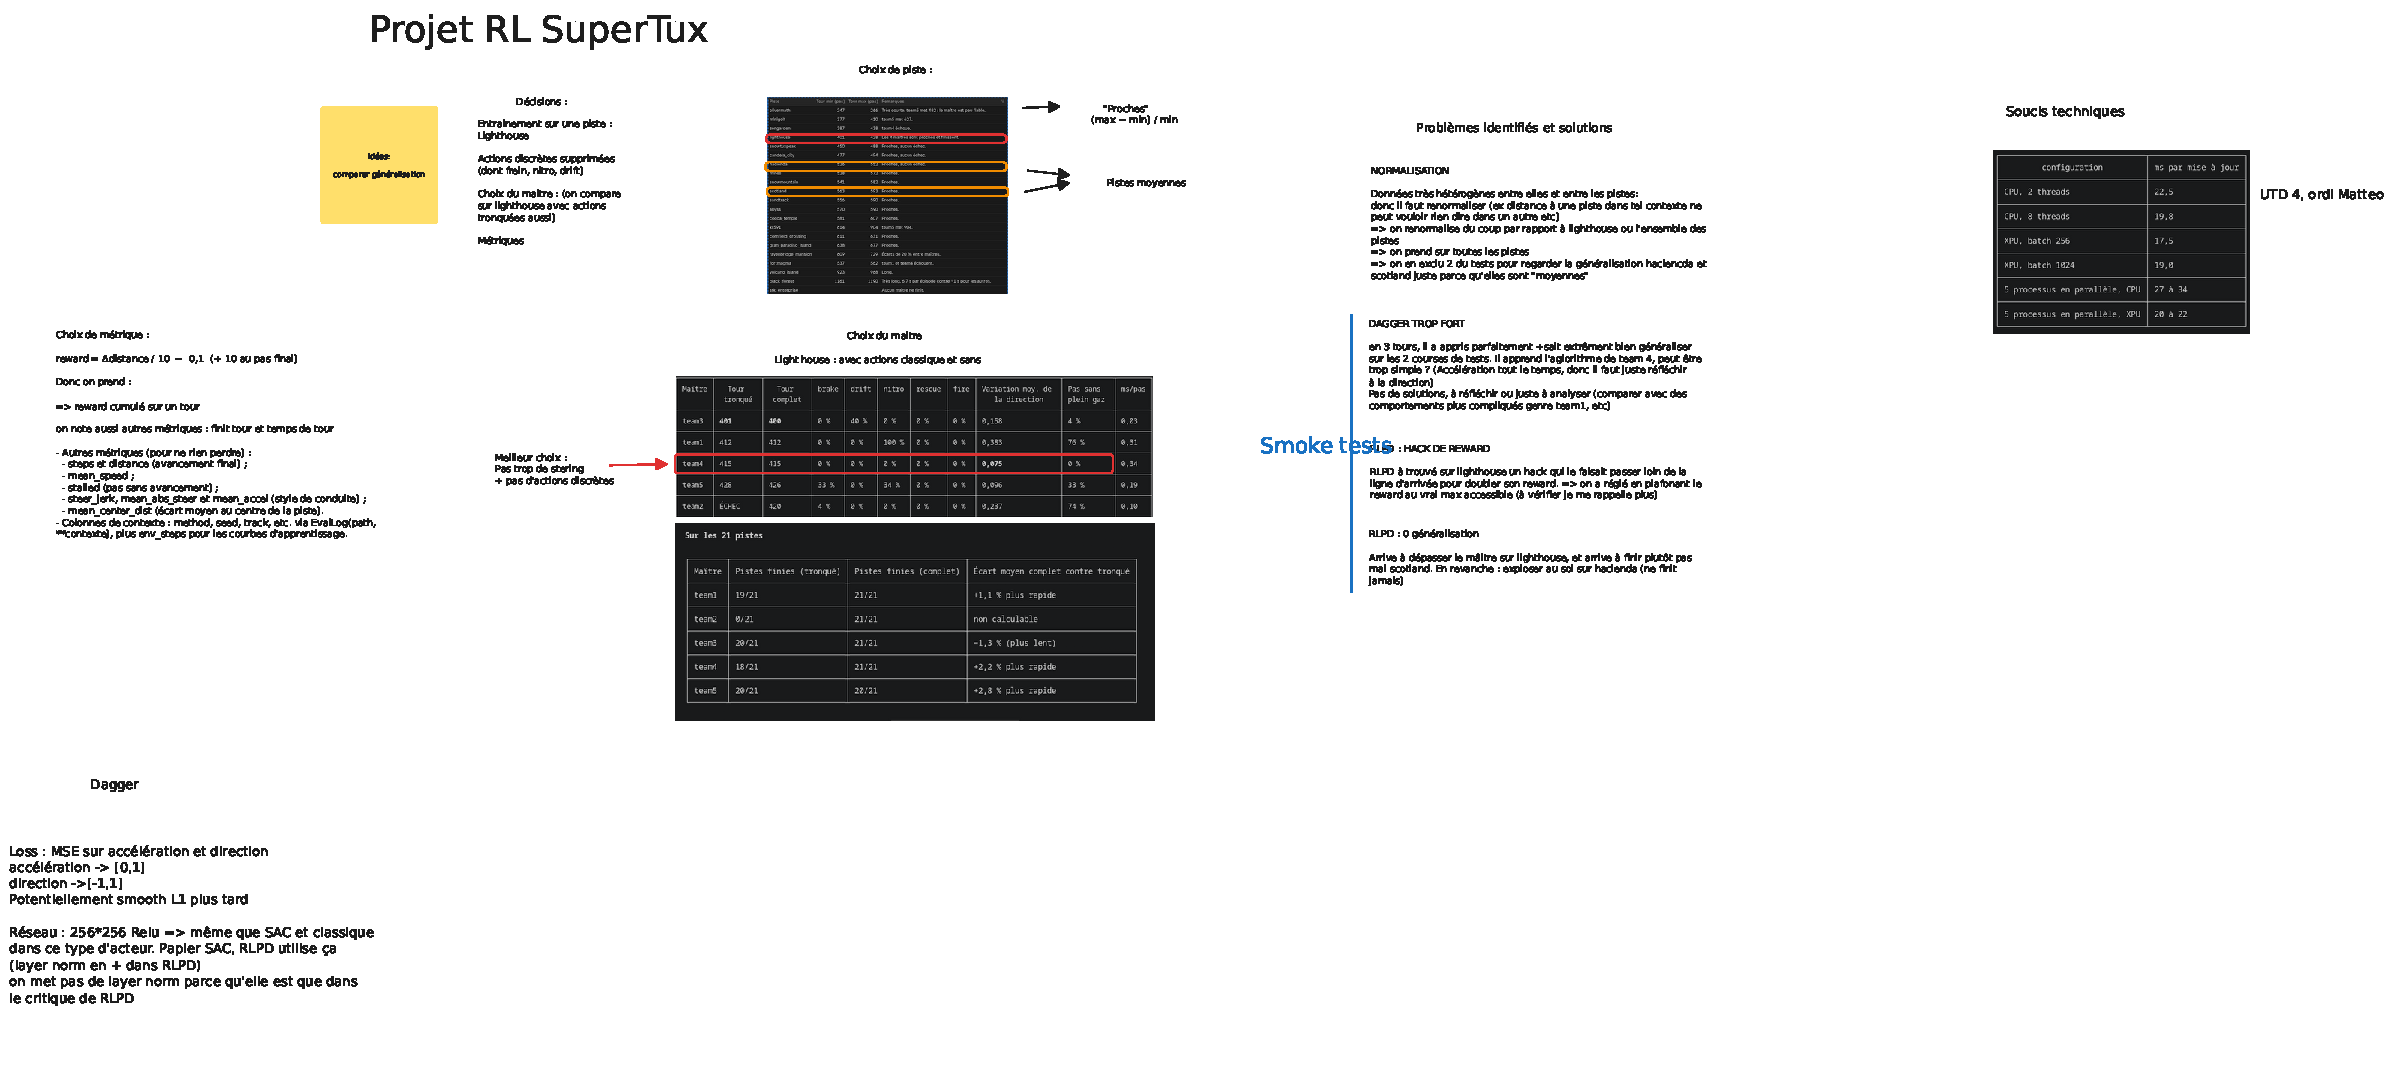
\includegraphics[width=\textwidth]{tableau.pdf}
  \caption{Our full brainstorm board (Excalidraw, in French): metric and DAgger settings, track and expert choice, problems found by the smoke
  tests and our answers, technical issues.}
  \label{fig:board}
\end{figure}

\begin{figure}[h]
\centering
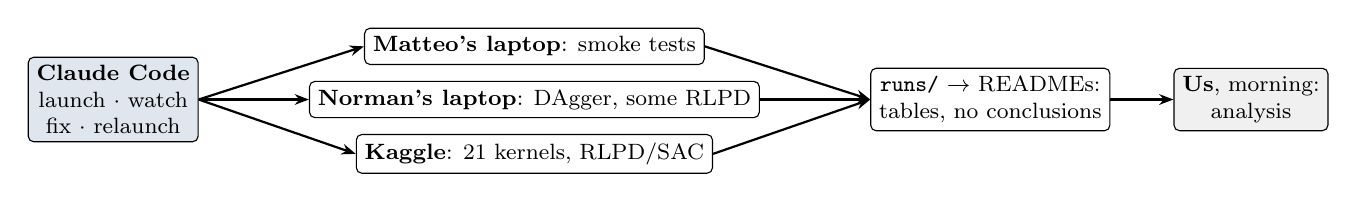
\begin{tikzpicture}[font=\footnotesize, node distance=2mm and 14mm,
  box/.style={draw, rounded corners=2pt, align=center, inner sep=3pt},
  pc/.style={box, minimum width=3.6cm},
  arr/.style={-{Stealth[length=1.8mm]}, thick}]
  \node[pc] (n) {\textbf{Norman's laptop}: DAgger, some RLPD};
  \node[pc, above=of n] (m) {\textbf{Matteo's laptop}: smoke tests};
  \node[pc, below=of n] (k) {\textbf{Kaggle}: 21 kernels, RLPD/SAC};
  \node[box, fill=navyblue!12, left=of n] (c) {\textbf{Claude Code}\\ launch $\cdot$ watch\\ fix $\cdot$ relaunch};
  \node[box, right=of n] (r) {\texttt{runs/} $\to$ READMEs:\\ tables, no conclusions};
  \node[box, right=8mm of r, fill=gray!12] (a) {\textbf{Us}, morning:\\ analysis};
  \foreach \x in {m, n, k} {\draw[arr] (c.east) -- (\x.west); \draw[arr] (\x.east) -- (r.west);}
  \draw[arr] (r) -- (a);
\end{tikzpicture}
\caption{Night of 12--13/11: Claude dispatches runs to three machines in parallel; all results land in the same \texttt{runs/} folder, about 180 runs.}
\label{fig:jobs}
\end{figure}

\end{document}
